\begin{pastexam}[label={px:gw3-103-ds-02}]{關務三等資訊處理 103 年 第二題}
（申論；20 分）

一個圖形（graph）包含五個頂點（vertex），$V_1, V_2, \ldots, V_5$，其鄰接矩陣（adjacency matrix）
\[
A = \begin{bmatrix}
0 & 1 & 3 & \infty & \infty \\
1 & 0 & 1 & 7 & 5 \\
3 & 1 & 0 & 6 & 2 \\
\infty & 7 & 6 & 0 & 3 \\
\infty & 5 & 2 & 3 & 0
\end{bmatrix}。
\]
\begin{itemize}[leftmargin=2.2em]
\item[㈠] 請使用 Floyd 的方法，計算此圖形的最短路徑長度矩陣（shortest path length matrix），來表示任兩頂點間最短
路徑長度。（10 分）
\item[㈡] 請使用 Prim 的方法，繪出此圖形的最小成本擴張樹（minimum cost spanning tree）。（5 分）
\item[㈢] 在任一圖形中，兩頂點在此圖形的最小成本擴張樹上的路徑，是否為這兩個頂點在此圖形上的最短路徑，請舉例
說明。（5 分）
\end{itemize}
\end{pastexam}

\begin{pastsoln}
答案：㈠ 最短路徑長度矩陣見下面的 $A^{5}$。 ㈡ 邊 $(V_1,V_2)$、$(V_2,V_3)$、$(V_3,V_5)$、$(V_5,V_4)$，總成本 $7$。
㈢ 不一定，例如三角形 $a$--$b$ 長 $2$、$b$--$c$ 長 $2$、$a$--$c$ 長 $3$。

矩陣是對稱的，這是一個無向圖，邊有 $(V_1,V_2)=1$、$(V_1,V_3)=3$、$(V_2,V_3)=1$、$(V_2,V_4)=7$、$(V_2,V_5)=5$、
$(V_3,V_4)=6$、$(V_3,V_5)=2$、$(V_4,V_5)=3$。

\textbf{㈠ Floyd 演算法}（資結書第~25.6~節）：$A^{k}[i][j]$ 是「中間只經過 $V_1, \ldots, V_k$」的最短路徑長度，
\[
A^{k}[i][j] = \min\bigl(A^{k-1}[i][j],\ A^{k-1}[i][k] + A^{k-1}[k][j]\bigr), \qquad A^{0} = A .
\]
每一輪把第 $k$ 列、第 $k$ 行當作跳板。 （粗體是這一輪變小的值。）
\[
A^{1} = \begin{bmatrix}
0 & 1 & 3 & \infty & \infty \\
1 & 0 & 1 & 7 & 5 \\
3 & 1 & 0 & 6 & 2 \\
\infty & 7 & 6 & 0 & 3 \\
\infty & 5 & 2 & 3 & 0
\end{bmatrix}
\quad
A^{2} = \begin{bmatrix}
0 & 1 & \mathbf{2} & \mathbf{8} & \mathbf{6} \\
1 & 0 & 1 & 7 & 5 \\
\mathbf{2} & 1 & 0 & 6 & 2 \\
\mathbf{8} & 7 & 6 & 0 & 3 \\
\mathbf{6} & 5 & 2 & 3 & 0
\end{bmatrix}
\quad
A^{3} = \begin{bmatrix}
0 & 1 & 2 & 8 & \mathbf{4} \\
1 & 0 & 1 & 7 & \mathbf{3} \\
2 & 1 & 0 & 6 & 2 \\
8 & 7 & 6 & 0 & 3 \\
\mathbf{4} & \mathbf{3} & 2 & 3 & 0
\end{bmatrix}
\]
\begin{itemize}
\item $k = 1$：經過 $V_1$ 沒有任何改善（$V_1$ 只連 $V_2$、$V_3$，而 $1 + 3 = 4 > A[2][3] = 1$），$A^{1} = A^{0}$。
\item $k = 2$：經過 $V_2$：$V_1 \to V_3$ 改成 $1 + 1 = 2$；$V_1 \to V_4$ 是 $1 + 7 = 8$；$V_1 \to V_5$ 是 $1 + 5 = 6$。
\item $k = 3$：經過 $V_3$：$V_1 \to V_5$ 改成 $2 + 2 = 4$；$V_2 \to V_5$ 改成 $1 + 2 = 3$。 （$V_1 \to V_4$ 經 $V_3$ 是
$2 + 6 = 8$，沒有變小。）
\item $k = 4$：經過 $V_4$ 沒有改善（例如 $V_1 \to V_5$ 經 $V_4$ 是 $8 + 3 = 11 > 4$），$A^{4} = A^{3}$。
\item $k = 5$：經過 $V_5$：$V_1 \to V_4$ 改成 $4 + 3 = 7$；$V_2 \to V_4$ 改成 $3 + 3 = 6$；$V_3 \to V_4$ 改成 $2 + 3 = 5$。
\end{itemize}
最短路徑長度矩陣：
\[
A^{5} = \begin{bmatrix}
0 & 1 & 2 & 7 & 4 \\
1 & 0 & 1 & 6 & 3 \\
2 & 1 & 0 & 5 & 2 \\
7 & 6 & 5 & 0 & 3 \\
4 & 3 & 2 & 3 & 0
\end{bmatrix}
\]
例如 $V_1$ 到 $V_4$ 最短是 $V_1 \to V_2 \to V_3 \to V_5 \to V_4$，$1 + 1 + 2 + 3 = 7$。

\textbf{㈡ Prim 演算法}（資結書第~24.3~節），從 $V_1$ 開始，每次加入一條連接「樹內」與「樹外」的最小邊：
\begin{enumerate}
\item 樹 $\{V_1\}$：候選 $(V_1,V_2)=1$、$(V_1,V_3)=3$，加入 $(V_1, V_2)$，成本 $1$。
\item 樹 $\{V_1, V_2\}$：候選 $(V_1,V_3)=3$、$(V_2,V_3)=1$、$(V_2,V_4)=7$、$(V_2,V_5)=5$，加入 $(V_2, V_3)$，成本 $1$。
\item 樹 $\{V_1, V_2, V_3\}$：候選 $(V_2,V_4)=7$、$(V_2,V_5)=5$、$(V_3,V_4)=6$、$(V_3,V_5)=2$，加入 $(V_3, V_5)$，成本 $2$。
\item 樹 $\{V_1, V_2, V_3, V_5\}$：候選 $(V_2,V_4)=7$、$(V_3,V_4)=6$、$(V_5,V_4)=3$，加入 $(V_5, V_4)$，成本 $3$。
\end{enumerate}
總成本 $1 + 1 + 2 + 3 = 7$。
\begin{center}
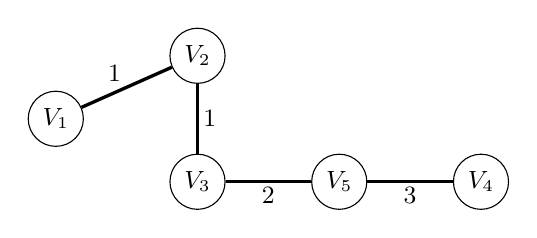
\begin{tikzpicture}[v/.style={circle,draw,minimum size=7mm,inner sep=0pt,font=\small},
  w/.style={font=\small,inner sep=1.5pt}]
\node[v] (1) at (0,0) {$V_1$};
\node[v] (2) at (1.8,0.8) {$V_2$};
\node[v] (3) at (1.8,-0.8) {$V_3$};
\node[v] (5) at (3.6,-0.8) {$V_5$};
\node[v] (4) at (5.4,-0.8) {$V_4$};
\draw[very thick] (1) -- node[w,above left] {1} (2);
\draw[very thick] (2) -- node[w,right] {1} (3);
\draw[very thick] (3) -- node[w,below] {2} (5);
\draw[very thick] (5) -- node[w,below] {3} (4);
\end{tikzpicture}
\end{center}
（每一步的最小邊都唯一，所以這棵最小成本擴張樹是唯一的。）

\textbf{㈢ 不一定。} 最小成本擴張樹讓\textbf{全部的邊加起來}最小，最短路徑讓\textbf{某兩點之間}的路徑最短，兩個目標不同
（資結書第~24.5.4~節）。 反例：三個頂點 $a, b, c$，邊 $(a,b) = 2$、$(b,c) = 2$、$(a,c) = 3$。 最小成本擴張樹選
$(a,b)$、$(b,c)$，成本 $4$；樹上 $a$ 到 $c$ 的路徑長 $2 + 2 = 4$，但圖上 $a$ 到 $c$ 直接走 $(a,c)$ 只要 $3$。
\begin{center}
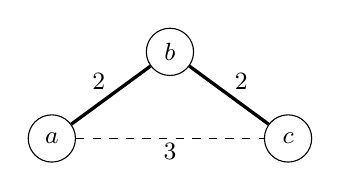
\begin{tikzpicture}[v/.style={circle,draw,minimum size=6mm,inner sep=0pt,font=\small},
  w/.style={font=\small,inner sep=1.5pt}]
\node[v] (a) at (0,0) {$a$};
\node[v] (b) at (1.5,1.1) {$b$};
\node[v] (c) at (3,0) {$c$};
\draw[very thick] (a) -- node[w,above left] {2} (b);
\draw[very thick] (b) -- node[w,above right] {2} (c);
\draw[dashed] (a) -- node[w,below] {3} (c);
\end{tikzpicture}
\end{center}
（粗線是最小成本擴張樹，虛線是不在樹上的邊。）本題的圖恰好每一對頂點在樹上的路徑都是最短路徑（和 $A^5$ 比對可知），
但這只是巧合，一般不成立。
\end{pastsoln}
